\documentclass[11pt,a4paper]{article}
\usepackage[utf8]{inputenc}
\usepackage[T1]{fontenc}
\IfFileExists{french.ldf}{\usepackage[french]{babel}}{\usepackage[english]{babel}}
\usepackage{amsmath,amssymb}
\usepackage{geometry}\geometry{margin=2.3cm}
\usepackage{xcolor}
\usepackage{enumitem}
\usepackage{graphicx}
\usepackage{wrapfig}
\usepackage{hyperref}
\hypersetup{colorlinks=true, urlcolor=[RGB]{2,101,115}, linkcolor=black}
\definecolor{teal}{RGB}{2,101,115}
\newcounter{tache}[section]
\newcommand{\T}[1][]{\refstepcounter{tache}\medskip\par\noindent\textbf{\thesection.\thetache}~\textit{#1}\quad}
\setlength{\parskip}{0.6em}
\usepackage{fancyhdr}\pagestyle{fancy}\fancyhf{}
\lhead{\small Agrégation --- Épreuve de modélisation --- Option B}
\rhead{\small Teneurs de marché automatisés}
\cfoot{\thepage}\renewcommand{\headrulewidth}{0.4pt}
\usepackage{titlesec}\titleformat*{\section}{\large\bfseries\color{teal}}
\titlespacing*{\section}{0pt}{1.6em}{0.6em}

\begin{document}

\begin{center}
{\large\bfseries Agrégation externe de mathématiques}\\[3pt]
{\bfseries Épreuve de modélisation --- Option B : calcul scientifique}\\[10pt]
\rule{0.85\linewidth}{0.4pt}\\[8pt]
{\LARGE\bfseries Dynamique d'un teneur de marché automatisé\\[2pt] à produit constant}\\[6pt]
{\itshape Formation des prix, glissement, perte impermanente et arbitrage}\\[8pt]
\rule{0.85\linewidth}{0.4pt}
\end{center}

\medskip
\begin{center}
\fbox{\begin{minipage}{0.95\linewidth}\small
Il est rappelé que le jury n'exige pas une compréhension exhaustive du texte. Vous êtes
laissé(e) libre d'organiser votre présentation comme vous l'entendez. Ce texte alterne des
\textbf{questions théoriques} (à démontrer) et des \textbf{tâches de simulation} (à programmer et à
illustrer). \textbf{Aucune réponse n'est fournie}~: il vous revient de conduire les démonstrations,
d'écrire les programmes et de produire les graphiques. Les figures ci-après indiquent seulement
\emph{l'allure attendue} des résultats de simulation~; elles servent de repère, non de correction.
Le jury appréciera que votre exposé s'appuie sur des \textbf{expériences numériques} menées sur
ordinateur (Python conseillé~: \texttt{numpy}, \texttt{matplotlib}).
\end{minipage}}
\end{center}

\bigskip
\section{Cadre et notations}

Un \emph{teneur de marché automatisé} (\emph{Automated Market Maker}, AMM) est un programme qui
échange automatiquement deux actifs $X$ et $Y$ à partir d'une \emph{réserve de liquidité}
contenant $x$ unités de $X$ et $y$ unités de $Y$. Il n'y a ni carnet d'ordres ni contrepartie
humaine~: le prix résulte d'une formule déterministe portant sur $(x,y)$. Le modèle dit
\emph{à produit constant} (popularisé par Uniswap~V2) impose l'invariant
\begin{equation}\label{eq:k}
  x\,y = k \quad (k>0 \text{ fixé, en l'absence d'apport ou de retrait de liquidité}).
\end{equation}
On note $p = y/x$ le \emph{prix instantané} d'une unité de $X$ en unités de $Y$. Un échange
consiste à apporter $\Delta x>0$ unités de $X$ à la réserve et à en retirer $\Delta y>0$ unités de
$Y$, de sorte que l'invariant~\eqref{eq:k} soit préservé. On travaillera en Python~3 avec
\texttt{numpy} et \texttt{matplotlib}. Sauf mention contraire, les échanges sont \emph{sans frais}.

Le texte comporte cinq parties largement indépendantes. Les trois premières mêlent théorie et
simulation déterministe~; la quatrième introduit une dynamique \emph{stochastique} (prix externe
aléatoire et arbitrage)~; la cinquième porte sur la \emph{validation numérique} des résultats. On
veillera, dans chaque simulation, à comparer les sorties numériques aux prédictions théoriques
établies, et à documenter les choix de discrétisation, de pas et de précision.

\medskip
\noindent\textbf{Objectifs de calcul scientifique.} Au-delà des réponses, on attend une réflexion
sur les \emph{méthodes}~: sommation contrôlée de séries et estimation de l'erreur de troncature~;
génération de nombres pseudo-aléatoires et estimateurs de Monte-Carlo~; vitesse de convergence
(géométrique pour les séries, en $1/\sqrt{N}$ pour Monte-Carlo)~; construction et lecture de
graphiques (échelles linéaire et semi-logarithmique, intervalles de confiance).

\section{Formation des prix et courbe d'échange}

\T[(théorie)] Montrer, à partir de l'invariant~\eqref{eq:k}, qu'un échange faisant passer la
réserve de $(x,y)$ à $(x+\Delta x,\, y-\Delta y)$ vérifie
\[
  \Delta y \;=\; \frac{y\,\Delta x}{x+\Delta x}.
\]
Préciser en quoi cette relation définit entièrement le comportement de l'AMM.

\T[(théorie)] Établir que le prix instantané $p=y/x$ après un tel échange est strictement
supérieur au prix instantané avant échange~: acheter du jeton $X$ en \emph{renchérit} le prix.

\T[(simulation)] Pour $k = 20\,000$, tracer la \emph{courbe d'échange} $\{(x,y):xy=k\}$ dans le
plan des réserves. Partant de l'état $(x,y)=(100,200)$, représenter graphiquement l'effet d'un
échange d'entrée $\Delta x=50$ (nouveau point de réserve et flèche de déplacement le long de la
courbe). Commenter la convexité de la courbe. \emph{L'allure attendue est donnée en Figure~1.}

\begin{figure}[h]\centering
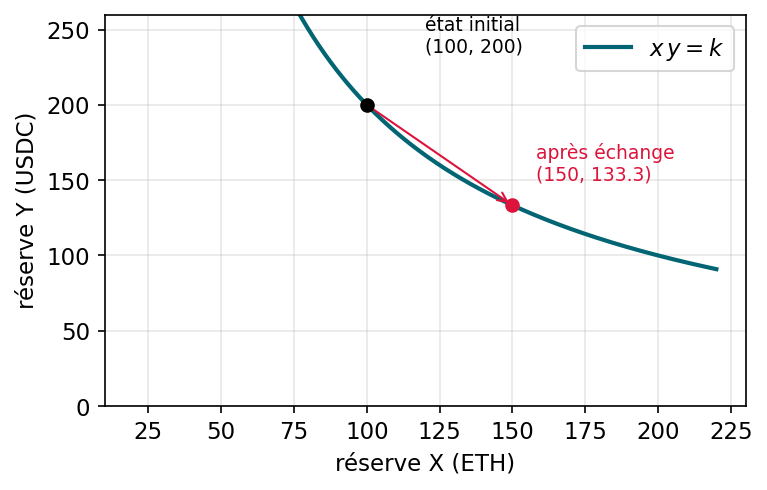
\includegraphics[width=0.80\linewidth]{figs/f1_hyperbole.png}
\caption{Allure attendue --- courbe à produit constant $xy=k$ et effet d'un échange (à reproduire).}
\end{figure}

\section{Bornes, monotonie et glissement}

On fixe une réserve $(x,y)$ et l'on étudie la fonction $\Delta x \mapsto \Delta y(\Delta x)$.

\T[(théorie)] Montrer que pour tout $\Delta x>0$ on a $\Delta y<y$ (la réserve de $Y$ ne peut
être entièrement vidée). Étudier la monotonie de $\Delta y(\Delta x)$ sur $]0,+\infty[$ et
déterminer sa limite en $+\infty$.

\T[(théorie)] Le \emph{prix effectif} d'un échange est $\pi(\Delta x)=\Delta x/\Delta y$.
L'exprimer en fonction de $x,y,\Delta x$, en déduire son sens de variation et sa limite lorsque
$\Delta x\to 0^{+}$. Interpréter le \emph{glissement} (\emph{slippage})~: écart entre prix
effectif et prix instantané.

\T[(simulation)] Pour $(x,y)=(100,100)$, tracer $\Delta y(\Delta x)$ pour $\Delta x\in[0,1000]$ et
faire apparaître l'asymptote. Superposer, sur un second graphique, le prix effectif
$\pi(\Delta x)$ et le prix instantané initial~; commenter la dégradation du prix avec la taille de
l'échange. \emph{L'allure attendue de la sortie $\Delta y$ est donnée en Figure~2.}

\begin{figure}[h]\centering
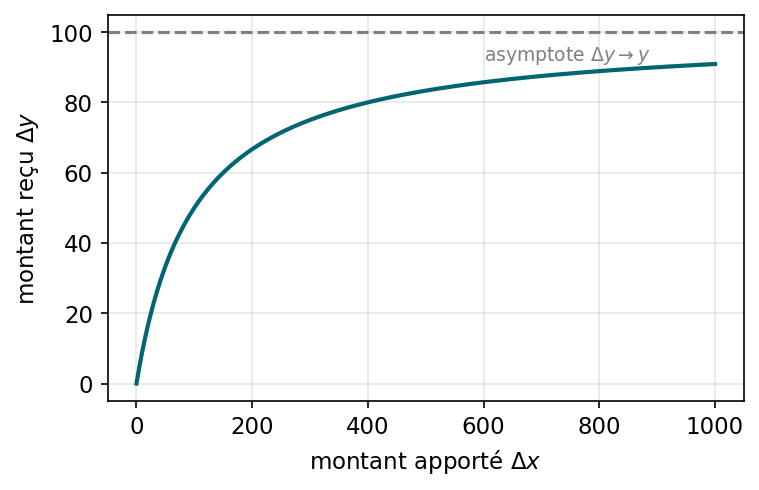
\includegraphics[width=0.78\linewidth]{figs/f2_sortie.png}
\caption{Allure attendue --- montant reçu $\Delta y$ en fonction du montant apporté $\Delta x$,
borné par la réserve $y$ (à reproduire).}
\end{figure}

\section{Frais cumulés : convergence et vitesse}

On modélise une longue séquence d'échanges dont les volumes décroissent géométriquement~: le
$i$-ième échange ($i\ge 0$) porte un volume $v_0\,\rho^{\,i}$ avec $0<\rho<1$, et prélève des
frais proportionnels de taux $f\in\,]0,1[$. On pose $\Phi_n=\sum_{i=0}^{n-1} f v_0 \rho^{\,i}$ et
$\Phi=\lim_{n\to\infty}\Phi_n$.

\T[(théorie)] Montrer que $\Phi$ est fini, en donner l'expression close, et majorer l'erreur
$\Phi-\Phi_n$ par une quantité géométrique en $\rho^{\,n}$. En déduire le nombre de termes
suffisant pour approcher $\Phi$ à une précision $\varepsilon$ donnée.

\T[(simulation)] Pour $f=0{,}003$, $v_0=1000$ et $\rho=0{,}9$, calculer numériquement les sommes
partielles $\Phi_n$ et les tracer en fonction de $n$, avec la valeur limite en repère. Sur un
second graphique en \emph{échelle semi-logarithmique}, tracer l'erreur $|\Phi-\Phi_n|$ et
vérifier expérimentalement le taux de convergence géométrique annoncé (droite de pente
$\log\rho$). \emph{L'allure attendue des sommes partielles est donnée en Figure~3.}

\begin{figure}[h]\centering
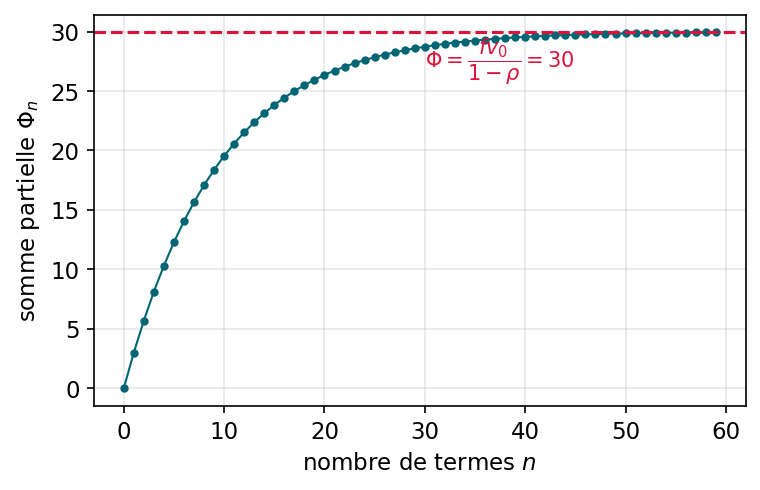
\includegraphics[width=0.78\linewidth]{figs/f4_series.png}
\caption{Allure attendue --- convergence des sommes partielles $\Phi_n$ vers $\Phi$ (à reproduire),
à compléter par le tracé semi-logarithmique de l'erreur.}
\end{figure}

\section{Perte impermanente et arbitrage stochastique}

Un \emph{fournisseur de liquidité} dépose $(x_0,y_0)$ dans la réserve, au prix initial
$p_0=y_0/x_0$. Le prix \emph{externe} du marché évolue ensuite et vaut $p_1=r\,p_0$
($r>0$). Des \emph{arbitragistes} échangent avec la réserve jusqu'à ce que le prix instantané du
pool coïncide avec le prix externe. On compare alors la valeur du dépôt \emph{resté dans la
réserve} à celle qu'il aurait eue \emph{conservé tel quel} (stratégie \guillemotleft~hold~\guillemotright)~:
l'écart relatif, toujours défavorable à la réserve, est la \emph{perte impermanente}
(\emph{impermanent loss}) $\mathrm{IL}(r)$.

\T[(théorie)] En utilisant l'invariant~\eqref{eq:k}, exprimer les réserves $(x_1,y_1)$ après
arbitrage en fonction de $k$ et du nouveau prix $p_1=r p_0$. En déduire une forme close de
$\mathrm{IL}(r)$, montrer que $\mathrm{IL}(1)=0$, que $\mathrm{IL}(r)\le 0$ pour tout $r>0$, et
étudier la symétrie de $\mathrm{IL}$ en fonction de $\log r$.

\T[(simulation)] Tracer $\mathrm{IL}(r)$ (en pourcentage) pour $r\in[1/4,\,4]$ et repérer son
maximum ($r=1$). \emph{L'allure attendue est donnée en Figure~4.} Vérifier numériquement la valeur
de $\mathrm{IL}$ pour un doublement ($r=2$) et un quadruplement ($r=4$) du prix.

\begin{figure}[h]\centering
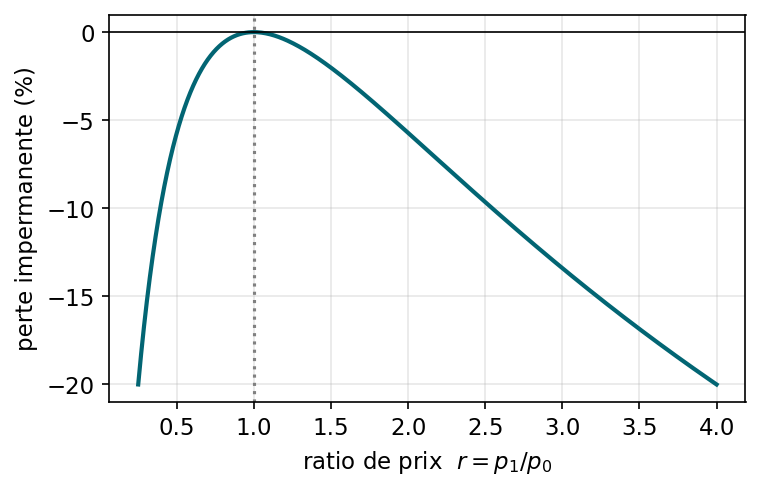
\includegraphics[width=0.78\linewidth]{figs/f3_il.png}
\caption{Allure attendue --- perte impermanente $\mathrm{IL}(r)$ en fonction du ratio de prix
$r=p_1/p_0$ (à reproduire).}
\end{figure}

\T[(simulation stochastique)] On simule le prix externe par une marche aléatoire multiplicative~:
$\log p_{t+1}=\log p_t+\sigma\,\xi_t$ où les $\xi_t$ sont i.i.d.\ $\mathcal{N}(0,1)$ et
$\sigma>0$. À chaque pas, on \emph{arbitre} la réserve pour aligner son prix sur $p_t$. Simuler,
sur un horizon $T=200$ et pour $\sigma=0{,}03$, la trajectoire du prix externe et celle de la
réserve $x_t$ qui en résulte (on prendra $x_0=y_0=100$, donc $k=10\,000$ et $p_0=1$). Superposer
plusieurs trajectoires et commenter le lien entre volatilité du prix et amplitude des variations
de réserve. \emph{L'allure attendue d'une trajectoire est donnée en Figure~5.}

\begin{figure}[h]\centering
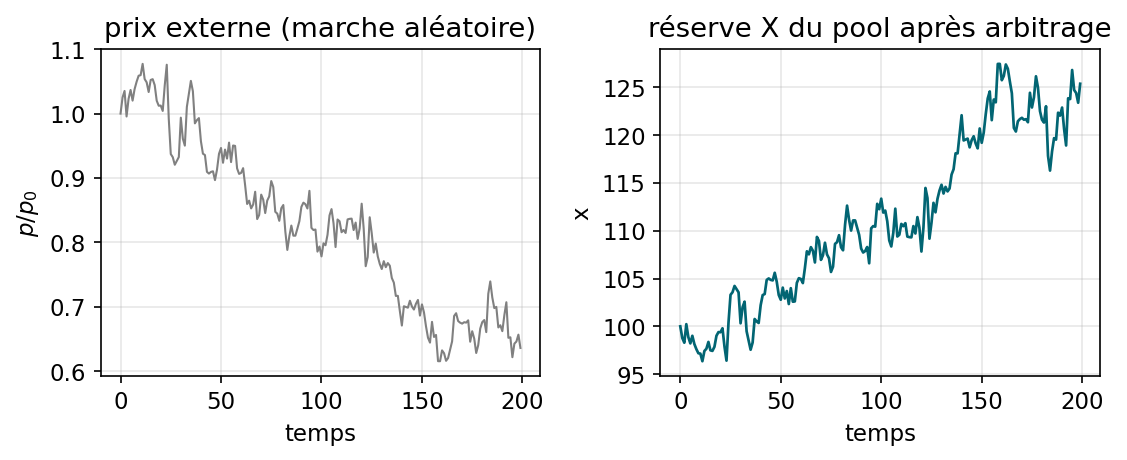
\includegraphics[width=0.98\linewidth]{figs/f5_arbitrage.png}
\caption{Allure attendue --- à gauche, un prix externe suivant une marche aléatoire~; à droite,
la réserve $x_t$ du pool après arbitrage à chaque pas (à reproduire).}
\end{figure}

\T[(simulation, Monte-Carlo)] Par une méthode de Monte-Carlo sur la marche aléatoire précédente,
estimer l'espérance de la perte impermanente $\mathbb{E}[\mathrm{IL}(p_T/p_0)]$ à l'horizon $T$,
en fonction de la volatilité $\sigma$. Tracer la courbe estimée $\sigma\mapsto
\mathbb{E}[\mathrm{IL}]$ avec ses intervalles de confiance, et confronter la tendance observée à
l'expression théorique de $\mathrm{IL}$ obtenue plus haut (développement au voisinage de $r=1$).

\section{Validation numérique et contrôle de l'erreur}

Cette partie invite à un regard critique sur la \emph{fiabilité} des simulations précédentes.

\T[(théorie \& simulation)] Pour l'estimateur de Monte-Carlo de $\mathbb{E}[\mathrm{IL}]$ de la
partie précédente, rappeler pourquoi l'erreur statistique décroît en $1/\sqrt{N}$ ($N$ étant le
nombre de tirages). Le vérifier expérimentalement en traçant, en échelle log-log, l'écart-type
empirique de l'estimateur en fonction de $N$, et en mesurant la pente obtenue.

\T[(simulation)] Proposer et mettre en \oe uvre une technique de \emph{réduction de variance}
(par exemple variables antithétiques sur les incréments $\xi_t$, ou variable de contrôle fondée
sur le développement de $\mathrm{IL}$ au voisinage de $r=1$). Comparer, à budget de calcul égal,
la largeur des intervalles de confiance avec et sans réduction de variance.

\T[(théorie)] Discuter la cohérence des unités et les cas limites~: comportement du modèle
lorsque $\Delta x\to 0$, lorsque $\rho\to 1^{-}$ (frais cumulés), et lorsque $\sigma\to 0$ (perte
impermanente). Ces limites sont-elles correctement reproduites par vos programmes~?

\section*{Prolongements possibles}

\emph{Pistes indépendantes, à explorer au gré de votre exposé~; il n'est pas demandé de les
traiter toutes.}
\begin{itemize}[nosep,leftmargin=1.3em]
  \item Comparer le modèle à produit constant $xy=k$ au modèle à \emph{somme constante} $x+y=k$
        et à la moyenne \guillemotleft~stable~\guillemotright{} de Curve~; discuter le glissement
        et le domaine de validité de chacun.
  \item Étudier l'effet des \emph{frais} sur l'arbitrage (bande de non-arbitrage) et sur la
        rentabilité du fournisseur de liquidité~: à partir de quel niveau de frais les frais
        compensent-ils la perte impermanente~?
  \item Analyser la sensibilité de $\mathbb{E}[\mathrm{IL}]$ à l'horizon $T$ et au pas de temps~;
        relier au mouvement brownien géométrique en temps continu.
  \item Discuter la précision et le coût des schémas numériques employés (sommation de séries,
        estimateurs de Monte-Carlo, réduction de variance).
\end{itemize}

\vfill
\noindent\rule{\linewidth}{0.3pt}\\
{\footnotesize\itshape Texte de modélisation (énoncé seul, sans corrigé) proposé dans le cadre
d'une préparation à l'agrégation par Pr Agrégé El Hadiq Zouhair --- \href{https://cpgeacademy.org}{cpgeacademy.org}.}

\end{document}
